\chapter{Programska podrška}

Prilikom razvoja programske podrške korišteno je integrirano razvojno okruženje \\ STM32CubeIDE, PDH sustav i programator ST-LINK/V2. Programska potpora razvijena je u jeziku C uz korištenje GCC prevodioca.

\section{Korišteni programski paketi i biblioteke}

Razvojno okruženje STM32CubeIDE nudi mogućnost grafičkog podešavanja parametara periferija i automatsko generiranje koda, čime su olakšane inicijalizacije raznih perifernih sklopova. Prije generiranja koda moguće je odabrati hoće li se koristiti HAL \engl{Hardware Abstraction Layer} ili LL \engl{Low-Layer} biblioteke.

HAL biblioteke nude visoku razinu abstrakcije i lakše su za koristiti, međutim, one rade po principu ,,crne kutije'', te ih stoga korisnik teže razumije. HAL biblioteke također zauzimaju više radne memorije od LL biblioteka jer u sebi sadržavaju kojekakve provjere vrijednosti i modifikacije unutarnjih HAL struktura, pa time nisu osigurane optimalne performanse.

Iz tog razloga odlučeno je da će se koristiti LL biblioteke. LL biblioteke omogućuju izravan pristup registrima periferija i korisnik ih daleko jednostavnije razumije, s obzirom na to da se često sastoje od samo jedne linije koda.

\section{Programska potpora za kameru}

Za rad s kamerom razvijene su korisničke funkcije prikazane u isječku koda \ref{lst:arducam_code}.

\begin{lstlisting}[caption=Korisničke funkcije za Arducam 5MP Mini Plus, label={lst:arducam_code}]
uint8_t ACAM_TestComms(void);
uint8_t ACAM_SPI_Read(uint8_t reg);
void ACAM_SPI_Write(uint8_t reg, uint8_t val);
void ACAM_spi_read_package(uint8_t * buff, uint16_t size);
void ACAM_I2C_Setup();
uint8_t ACAM_I2C_Read(uint16_t reg);
void ACAM_I2C_Write(uint16_t reg, uint8_t command);
void ACAM_I2C_WriteSeq(const struct ACAM_I2C_Register commandSeq[]);
uint8_t ACAM_TestComms(void);
void ACAM_select_JPEG(void);
void ACAM_select_RAW(uint8_t resolution);
void ACAM_start_capture(void);
uint32_t ACAM_get_image_size();
void ACAM_set_exposure(uint16_t nr_lines, uint8_t nr_lines_frac);
void ACAM_Reset(void);
void ACAM_exp_gain_manual(void)
void ACAM_exp_gain_auto(void)
uint8_t ACAM_is_cap_complete(void)
void ACAM_set_gain(uint8_t gain);
\end{lstlisting}

\noindent Za testiranje SPI i I\textsuperscript{2}C komunikacije između mikrokontrolera i kamere postoji funkcija \verb|ACAM_TestComms()|, za odabir između RAW i JPEG formata slike na raspolaganju su funkcije \verb|ACAM_select_RAW()| i \verb|ACAM_select_JPEG()|. Način upravljanja ekspozicijom odabire se funkcijama \verb|ACAM_exp_gain_manual()| i \\ \verb|ACAM_exp_gain_auto()|, a ukoliko se odabere ručni način upravljanja ekspozicijom parametri vremena ekspozicije i pojačanja pojačala se podešavaju funkcijama \verb|ACAM_set_exposure()| i \verb|ACAM_set_gain()|. Komanda za početak slikanja se šalje funkcijom \\ \verb|ACAM_start_capture()|, a provjera završetka slikanja se obavlja funkcijom \\ \verb|ACAM_is_cap_complete()|. Navedene funkcije nije trebalo mijenjati u odnosu na prethodnu programsku podršku, pa one rade na isti način kao i u prethodnom radu \cite{diplomski_goran_petrak}. Funkcije koje direktno rade sa SPI i I\textsuperscript{2}C periferijom su jedine mijenjane s obzirom na to da se rad periferija između prethodno korištenog i trenutačno korištenog mikrokontrolera razlikuju, kako je i pokazano u poglavlju 3. U nastavku će biti istaknute razlike između starih i novih funkcija kao i obrazloženje radi čega je došlo do promjena.

\subsection{Funkcije za rad sa I\textsuperscript{2}C periferijom}

Funkcije za rad s I\textsuperscript{2}C periferijom navedene su u isječku koda \ref{lst:acam_i2c_functions}.

\begin{lstlisting}[caption=Funkcije za rad s I\textsuperscript{2}C periferijom, label={lst:acam_i2c_functions}]
void ACAM_I2C_Setup();
uint8_t ACAM_I2C_Read(uint16_t reg);
void ACAM_I2C_Write(uint16_t reg, uint8_t command);
void ACAM_I2C_WriteSeq(const struct ACAM_I2C_Register commandSeq[]);
\end{lstlisting}

\noindent U odnosu na prethodnu programsku podršku dodana je funkcija \verb|ACAM_I2C_Setup()| koja podešava I\textsuperscript{2}C periferiju. Funkcija postavlja adresu uređaja s kojim se želi komunicirati, odnosno SADD registar, i govori periferiji želi li se na uređaj nešto čitati ili pisati, odnosno podešava RD\_WRN bit u I2C\_CR2 registru. Tu funkciju je važno pozvati prije svakog pokušaja komunikacije s kamerom. Funkcije \verb|ACAM_I2C_Write()|,  \verb|ACAM_I2C_Read()| i \verb|ACAM_I2C_WriteSeq()| služe za prijenos podataka između kamere i mikrokontrolera, i one su prošle manje promjene, konkretno, bilo je potrebno omogućiti drugačije prekide i provjeravati drugačije statusne zastavice, zato što registarska mapa I\textsuperscript{2}C periferije izgleda drugačije na STM32L471VGT6 mikrokontroleru nego na STM32F407VGT6 mikrokontroleru. Navedene promjene nije bilo teško implementirati zato što LL funkcije koriste intuitivna imena. Na primjer, funkcija koja omogućava TC prekid (prekid za završetak prijenosa) je \verb|LL_I2C_EnableIT_TC()|, a funkcija koja provjerava da li je podignuta zastavica BUSY (prijenos je u tijeku) je \verb|LL_I2C_IsActiveFlag_Busy()|.

Prijenos preko I\textsuperscript{2}C protokola u ovom radu funkcionira tako da se u jednoj od funkcija koje su zadužene za prijenos podataka postavi adresa uređaja s kojim se želi komunicirati (u ovom slučaju kamera), nakon toga generira se \textit{start} uvjet i omogućuju se prekidi relevantni za vrstu prijenosa koja se želi obaviti (slanje ili primanje podataka). Stanje komunikacije se prati preko globalne zastavice koja se osvježava u prekidnoj podrutini \verb|I2C1_EV_IRQHandler()|. Jedina promjena koju je prekidan funkcija doživjela jest ta da je izbrisan kod za provjeru je li poslana adresa \textit{slave} uređaja. Naime, na prethodno korištenom mikrokontroleru nije postojao posebni registar za adresu \textit{slave} uređaja, nego se adresa slala preko izlaznog registra periferiju. Kod novog mikrokontrolera, čim se pošalje \textit{start} bit šalje se adresa \textit{slave} uređaja preko SADD registra i automatski se provjerava da ACK bit za potvrdu primitka točne adrese \textit{slave} uređaja. Ostatak funkcije funkcionira na isti način kao i na prethodnom mikrokontroleru.

\subsection{Funkcije za rad sa SPI periferijom}

Funkcije za rad s SPI periferijom navedene su u isječku koda \ref{lst:acam_spi_functions}.

\begin{lstlisting}[caption=Funkcije za rad s SPI periferijom, label={lst:acam_spi_functions}]
uint8_t ACAM_SPI_Read(uint8_t reg);
void ACAM_SPI_Write(uint8_t reg, uint8_t val);
void ACAM_spi_read_package(uint8_t * buff, uint16_t size);
\end{lstlisting}

\noindent Kao što je već rečeno, SPI periferija funkcionira na isti način na oba mikrokontrolera, te stoga funkcije \verb|ACAM_SPI_Read()| i \verb|ACAM_SPI_Write()| funkcioniraju na isti način kao i u programskoj podršci za prethodni mikrokontroler.

Do razlike, međutim, dolazi u funkciji \verb| ACAM_spi_read_package()|, jer ta funkcija koristi DMA prijenos, a kao što je već pokazano, DMA prijenos funkcionira drugačije na STM32L471VGT6 mikrokontroleru nego na STM32F407VGT6 mikrokontroleru. U prethodnoj programskoj podršci koristili su se takozvani tokovi kod DMA prijenosa. Na primjer, za slanje podataka preko SPI protokola pomoću DMA prijenosa koristio se tok 4, a u programskoj podršci tok 4 je označavala definicija \verb|LL_DMA_STREAM_4|. U programskoj podršci za trenutačni mikrokontroler ne postoje takve definicije za tokove, s obzirom na to da se prijenos obavlja preko takozvanih kanala. Ako se žele poslati podatci preko SPI protokola pomoću DMA prijenosa mora se koristiti kanal 5, a za primanje podataka koristi se kanal 4, a u programskoj podršci kanale 4 i 5 predstavljaju definicije \verb|LL_DMA_CHANNEL_4| i \verb|LL_DMA_CHANNEL5|. Navedene promjene bilo je jednostavno implementirati jer se koriste globalne definicije preko kojih se programskoj podršci govori koje dijelove periferije se koriste, tako da je bilo potrebno promijeniti svega nekoliko linija koda (isječak koda \ref{lst:global_dma_def}).
\begin{lstlisting}[caption=Zaglavlje \texttt{dma.h} datoteke u kojima se definira koji dijelovi periferija se koriste, label={lst:global_dma_def}]
#define ACAM_SPIn	SPI2

#define ACAM_LL_DMA_CHANNEL_TX	LL_DMA_CHANNEL_5
#define ACAM_LL_DMA_CHANNEL_RX	LL_DMA_CHANNEL_4

#define ACAM_DMA_CHANNEL_TX_IRQn	DMA1_Channel5_IRQn
#define ACAM_DMA_CHANNEL_RX_IRQn	DMA1_Channel4_IRQn

#define ACAM_DMAn	DMA1
\end{lstlisting}

Konačno, trebalo je izbrisati funkcije koje se bave prekidima koji ne postoje na trenutačnom mikrokontroleru i prilagoditi prekidne funkcije da rade s prekidima kanala 4 i 5. Na primjer, kod STM32L471VGT6 mikrokontrolera ne postoje DMEIF i FEIF zastavice, pa je, na primjer, funkcije \verb|LL_DMA_ClearFlag_DMEx()| i \\ \verb|LL_DMA_ClearFlag_FEx()| jednostavno bilo potrebno izbrisati (x u nazivu funkcije može biti 3 ili 4, što predstavlja broj toka). Funkcije koje rade s HT, TC i TE prekidima, na primjer \verb|LL_DMA_ClearFlag_HTx()|, \verb|LL_DMA_ClearFlag_TCx()| i \\ \verb|LL_DMA_ClearFlag_TEx()|, je trebalo promijeniti da rade s brojem kanala koji se koriste, a to znači promijeniti x u 4 ili 5, što predstavlja broj kanala. Na isti način modificirane su druge funkcije koje rade s prekidima kanala

Na taj je način postojeća programska podrška prethodnog mikrokokontrolera za kameru prilagođena za trenutačni mikrokontroler.

\section{Programska potpora za \textit{flash} memoriju}

%\subsection{Funkcije za rad s \textit{flash} memorijom}

Za rad s \textit{flash} memorijom razvijene su korisničke funkcije prikazane u isječku koda \ref{lst:flash_code}.

\begin{lstlisting}[caption=Korisničke funkcije za \textit{flash} memoriju, label={lst:flash_code}]
uint8_t W25N_init(void);
uint8_t W25N_block_erase(uint16_t block_nr);
uint8_t W25N_page_data_read(uint16_t page_addr);
uint8_t W25N_read_data(uint16_t col_addr, uint8_t * data, uint16_t nr_bytes);
uint8_t W25N_prog_data_load(uint16_t col_addr, uint8_t * data, uint16_t nr_bytes);
uint8_t W25N_rand_prog_data_load(uint16_t col_addr, uint8_t * data, uint16_t nr_bytes);
uint8_t W25N_prog_execute(uint16_t page_addr);
\end{lstlisting}

\noindent Inicijalizacija perifernih jedinica potrebnih za rad s \textit{flash} memorijom, provjera ispravnosti SPI komunikacije izvršava se funkcijom \verb|W25N_init()|. Brisanje bloka izvršava se funkcijom \verb|W25N_block_erase()|. Prebacivanje odabrane stranice u međuspremnik \textit{flash} memorije izvodi se pomoću funkcije \verb|W25N_page_data_read()|, a nakon toga željeni niz okteta se može pročitati funkcijom \verb|W25N__read_data()|. Funkcijama \verb|W25N_prog_data_load()| i \verb|W25N_rand_prog_data_load()| izvodi se upisivanje u međuspremnik. Funkcija \verb|W25N_prog_execute()| upisuje podatke iz međuspremnika u stranicu u memoriji.

Funkcije koje još rade sa \textit{flash} memorijom su one koje upravljaju neispravnim blokovima (isječak koda \ref{lst:block_man}).

\begin{lstlisting}[caption=Funkcije za upravljanje neispravnim blokovima, label={lst:block_man}]
void W25N_scan_factory_BB(uint32_t * BBBT);
void W25N_bb_manage(uint16_t lba, uint16_t pba);
void W25N_read_bbm_lut(uint8_t * container);
\end{lstlisting}

\noindent Funkcija \verb|W25N_scan_factory_BB()| skenira blokove u tablici bitova i označuje one koji su tvornički neispravni, a tablica bitova koju treba skenirati dobiva preko pokazivača \verb|BBBT|. Funkcija \verb|W25N_bb_manage()| omogućuje specificiranje zamjenskog bloka za blok koji je uočen kao neispravan. Funkcijom \verb|W25N_read_bbm_lut()| se iščitava prozivna tablica (LUT), čime se dobivaju adrese neispravnih i zamjenskih blokova.

Zajedničko svim prethodnim funkcijama je korištenje funkcije prikazane u isječku koda \ref{lst:flash_execute}.

\begin{lstlisting}[caption=Funkcija za izvođenje instrukcije na \textit{flash} memoriji, label={lst:flash_execute}]
void W25N_instruction_execute( W25N_instruction_nr instr, uint8_t *params, uint8_t *data_or_rbs, uint32_t nr_data_bytes);
\end{lstlisting}

\noindent Funkcija \verb|W25N_instruction_execute()| se izvršavaju instrukcije na \text{flash} memoriji i ona radi direktno s registrima SPI periferije. U ovoj funkciji su jedino nastajali problemi, a greška se događala kod upisa u podatkovni registar SPI periferiji. Na primjer, ako se želi poslati neki podatak preko SPI protokola, željeni podatak potrebno je upisati u registar SPI1\_DR, a način na koji se je to radilo u prethodnoj programskoj prikazan je u isječku koda \ref{lst:spi_dr_old}.

\begin{lstlisting}[caption=Upis podatka u SPI2\_DR registar, label={lst:spi_dr_old}]
SPI1->DR = 0x69;
\end{lstlisting}

\noindent Naime, SPI komunikacija u ovom projektu radi s 8-bitnim podatcima, međutim, promatranjem linije kroz osciloskop, primijećeno je da se šalje 16-bitni podatak, s tim da se traženi podatak nalazi u gornja dva bajta. Ovaj problem riješen je korištenjem odgovarajuće LL funkcije, a u slučaju slanja podatka, primjer u isječku koda \ref{lst:spi_dr_old} prikazan je na ispravno napisan način u isječku koda \ref{lst:spi_dr_new}.

\begin{lstlisting}[caption=Ispravan upis podatka u SPI2\_DR registar, label={lst:spi_dr_new}]
LL_SPI_TransmitData8(SPI1, 0x69);
\end{lstlisting}

\section{Integracija s operacijskim sustavom FreeRTOS}

Za povezivanje razvijene programske potpore i ostvarivanja višezadaćnosti korišten je operacijski sustav za rad u stvarnom vremenu FreeRTOS. Razvijeni su zadaci \textit{Camera Task} za upravljanje kamerom i \textit{XBand \& MemMang Task} za upravljanje memorijom i slanjem podataka preko USART sučelja na računalo u svrhu demonstracije. \textit{Interpreter task} zadatak služi za upravljanje ostalim zadacima. Preko \textit{Interpreter} zadatka zadaju se parametri koje će koristiti kamera (vrijeme ekspozicije, pojačanje i format) kao imena datoteka u koje će se spremiti slika (imena imaju nazive brojeva u intervalu od 0 do 1023). Preko \textit{Interpreter} zadatka se također može odabrati datoteka za slanje preko USART sučelja, a željena datoteka se može i izbrisati. Također, ako je došlo do nekakvih problema, moguće je ponovno inicijalizirati datotečni sustav \textit{flash} memorije.
Prikaz zadataka u obliku blok dijagrama prikazan je na slici \ref{fig:tasks}.

\begin{figure}[H]
	\centering
	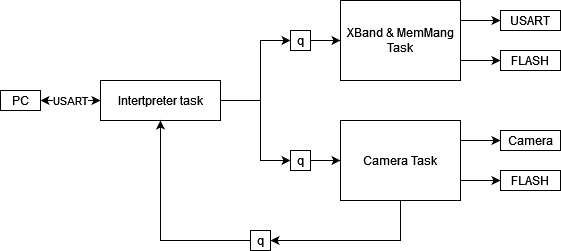
\includegraphics[width=\textwidth]{damn_rtos.png}
	\caption{Zadaci u operacijskom sustavu PDH računala}
	\label{fig:tasks}
\end{figure}

\noindent Dio programa koji uzima i sprema sliku, kao i dio programa koji šalje podatke na USART sučelje, predstavljaju kritične sekcije, jer bi njihovo prekidanje moglo dovesti do grešaka pri upravljanju s podacima.

\section{Programska podrška za CAN komunikaciju}

S obzirom na neispravnost sklopa za CAN komunikaciju na tiskanoj pločici PDH sustava, programska podrška za CAN sučelje nije razvijena. Ipak, u ovom poglavlju dat će se pregled funkcija koje će se najčešće koristiti jednom kada se programska podrška počne razvijati. Za razliku od ostalih sučelja na STM32L471VGT6 mikrokontroleru ne postoje LL biblioteke koje rukuju CAN periferijom, pa će se stoga koristiti HAL biblioteke.

\subsection{Inicijalizacija}

Konfiguracija CAN periferije može se izvesti korištenjem generatora koda u \\STM32CubeIDE razvojnom okruženju, a prikaz osnovne konfiguracije prikazan je na slici \ref{fig:can_config}.

\begin{figure}[H]
	\centering
	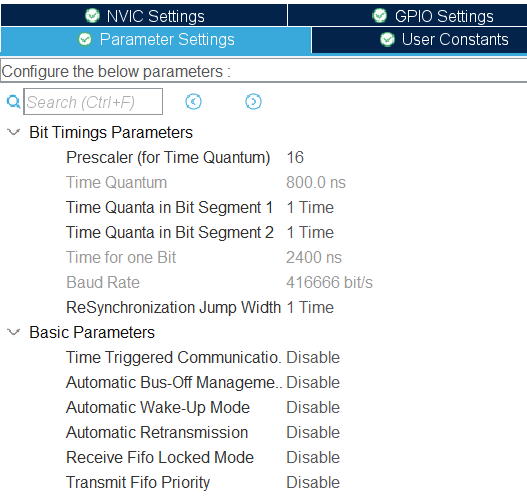
\includegraphics[width=\textwidth]{can_config.png}
	\caption{Konfiguracija CAN periferije}
	\label{fig:can_config}
\end{figure}

\noindent Generator koda će napraviti kod za inicijalizaciju CAN periferije implementiranjem \verb|HAL_CAN_MspInit()| funkcije, u kojoj se omogućuje takt za CAN sučelje, podešavaju se stezaljke koje će CAN koristiti i omogućit će i podesiti prioritete prekida. CAN periferija će se inicijalizirati preko \verb|HAL_CAN_Init()| funkcije koja koristi \verb|HAL_CAN_MspInit()| funkciju za \textit{low-level} inicijalizaciju.

Generator koda ne nudi opciju konfiguracije filtra, pa stoga korisnik mora sam implementirati funkciju za konfiguraciju filtra \verb|HAL_CAN_ConfigFilter()|, čiji je prototip dan u isječku koda \ref{lst:filter_config_prototype}.

\begin{lstlisting}[caption=Prototip funkcije \texttt{HAL\_CAN\_ConfigFilter()}, label={lst:filter_config_prototype}]
HAL_StatusTypeDef HAL_CAN_ConfigFilter(CAN_HandleTypeDef *hcan, const CAN_FilterTypeDef *sFilterConfig)
\end{lstlisting} 

\noindent Funkcija prima pokazivač na strukturu \verb|*sFilterConfig|, koja sadržava željene parametre filtra. Kako bi se filter podesio, korisnik prvo treba napraviti strukturu tipa \verb|CAN_FilterTypeDef| koja sadržava sve potrebne parametre filtra (isječak koda \ref{lst:can_filtertypedef}).

\begin{lstlisting}[caption=\texttt{CAN\_FilterTypeDef} struktura, label={lst:can_filtertypedef}]
typedef struct
{
  uint32_t StdId;
  uint32_t ExtId;
  uint32_t IDE;
  uint32_t RTR;
  uint32_t DLC;
  FunctionalState TransmitGlobalTime;

} CAN_TxHeaderTypeDef;
\end{lstlisting}

\noindent Kada se napravi inicijalizacija, CAN modul se uključuje \verb|HAL_CAN_Start()| funkcijom. Čvor je sada aktivan na sabirnici i može primati i slati poruke.

\subsection{Korištenje}

Slanjem poruka se upravlja sljedećim funkcijama:
\begin{itemize}
	\item \verb|HAL_CAN_AddTxMessage()| - zahtjev za slanjem nove poruke,
	\item \verb|HAL_CAN_AbortTxRequest()| - zahtjev za prekidom poruke u tijeku slanja,
	\item \verb|HAL_CAN_GetTxMailboxesFreeLevel()| - vraća broj slobodnih odašiljačkih \textit{mailbox} struktura,
	\item \verb|HAL_CAN_IsTxMessagePending()| - provjerava da li je poruka u tijeku slanja
	\item \verb|HAL_CAN_GetTxTimestamp()| - vraća vremensku oznaku poslane poruke, u slučaju da je omogućen način rada s vremenski okinutom komunikacijom.
\end{itemize}
\noindent Poruka primljena u FIFO strukturi se može pročitati \verb|HAL_CAN_GetRxMessage()| funkcijom, broj poruka pohranjenih u FIFO strukturi se može dobiti preko funkcije \verb|HAL_CAN_GetRxFifoFillLevel()|.

Primanje i slanje podataka se može izvoditi preko prekida, koji se mogu uključiti funkcijom \verb|HAL_CAN_ActivateNotification()|. CAN periferija se može prebaciti u način rada s niskom potrošnjom energije uz pomoć \verb|HAL_CAN_RequestSleep()| funkcije, a povratak u normalan način rada ostvaruje funkcija \verb|HAL_CAN_WakeUp()|.

\section{Učitavanje programa}

Kako bi se programska podrška mogla učitati na mikrokontroler PDH sustava nužno je koristiti programator, u ovom slučaju ST-LINK/V2. Na raspolaganju je \\ STM32F4DISCOVERY razvojni sustav koji ima ugrađen ST-LINK/V2 programator. Programator na razvojnom sustavu se može koristiti za programiranje mikrokontrolera na razvojnom sustavu ili programiranje mikrokontrolera na vanjskoj pločici. Koji mikrokontroler programator programira određuju prespojnici CN3 na razvojnom sustavu:
\begin{itemize}
	\item ako su oba prespojnika spojena, programira se mikrokontroler na razvojnom sustavu,
	\item ako su oba prespojnika odspojena, programira se mikrokontroler na vanjskoj pločici.
\end{itemize}
Programiranje se izvodi preko CN2 konektora na razvojnom sustavu i X6 konektora na PDH sustavu. Funkcije stezaljki na pojedinim konektorima su dane u tablici \ref{Tab:conn_func}.
\begin{center}
	\begin{table}[H]
		\centering
		\caption{Opis stezaljki CN2 i X6 konektora \cite{zavrsni_filip_juric}, \cite{disc_manual}}
		\begin{tabular}{| c | c | c |}
			\hline
			Redni broj stezaljke & CN2 & X6 \\
			\hline
			1. & VDD & VDD \\
			\hline
			2. & SWCLK & SWDIO \\
			\hline
			3. & GND & SWCLK \\
			\hline
			4. & SWDIO & SWO \\
			\hline
			5. & NRST & NRST \\
			\hline
			6. & SWO & GND \\
			\hline
		\end{tabular}
		\label{Tab:conn_func}
	\end{table}
\end{center}
Potrebno je spojiti istoimene stezaljke kako bi se učitavanje programa uspješno izvelo. Osim za programiranje, razvojni sustav se koristi kao izvor napajanja za PDH računalo, s obzirom na to da sustav napajanja na PDH sustavu trenutačno nije ispravan.